\documentclass [11pt, proquest] {uwthesis}[2020/02/24]
\usepackage{graphicx}
\graphicspath{ {./images/} }

\setcounter{tocdepth}{1}  % Print the chapter and sections to the toc

\let\mffont=\sf

\begin{document}

\prelimpages

\Title{Securing WireGuard private keys with a hardware token\\}
\Author{Peter Van Eenoo}
\Year{2022}
\Program{Computer Science and Engineering}

\Chair{Brent Lagesse}{Dr.}{Computing \& Software Systems}
\Signature{William Erdly}
\Signature{Yang Peng}

\copyrightpage

\titlepage  


\setcounter{page}{-1}
\abstract{

WireGuard is a popular, secure, and relatively new VPN implementation that has seen widespread adoption. WireGuard's non-traditional key management in its reference implementation, poses some weaknesses that could be exploited by malware to find and exfiltrate keys, compromising a user's identity. WireGuard's use of Curve25519 keys for identity and authentication, posed a challenge to me due to its lack of mature security key support. In this project, I modified WireGuard to use the PKCS\#11 interface in order to securely store a user's private and public key on a USB security key. Using a comparative threat model analysis, I show how my modifications improve the security of the system and decrease the attack surface of WireGuard. My modifications make WireGuard more immune to malware and threat actors while allowing a user to 'carry' their identify with them and move between machines without copying files.

}

\tableofcontents
\listoffigures

\chapter*{Glossary}      % starred form omits the `chapter x'
\addcontentsline{toc}{chapter}{Glossary}
\thispagestyle{plain}

\begin{glossary}

\item[WireGuard]

a VPN technology created in 2017 by Jason DonenFeld that operates at the network layer. It aims to be a replacement for popular TLS-based VPNs like OpenVPN and IPsec. WireGuard uses a fixed-set of cryptographic primitives and by design, has no support for negotiation of these primitives. 

\item[Curve25519]
an elliptic curve with a 256-bit key size. Designed by Daniel J. Bernstein in 2005\cite{noauthor_curve25519_nodate}. 
Curve25519 has a digital signature algorithm named Ed25519 and a key derivation algorithm named X25519.

\item[X25519]
a key exchange algorithm that uses Curve25519 to implement Elliptic-curve Diffie–Hellman (ECDH) key exchange. This process is also known as a key derivation function (KDF).

\item[Ed25519] a digital signature algorithm that uses the Curve25519.

\item[AEAD]
Authenticated encryption with additional data. A class of encryption algorithms which enforce confidentiality and authenticity of data. 

\item[ChaCha20Poly1350]
an AEAD encryption algorithm which is composed of the ChaCha20 stream cipher and Poly1305 for message authentication code (MAC)

\item[PKCS\#11] a public-key cryptography standard governed by the OASIS technical committee\cite{noauthor_cryptsoft_nodate} that defines a common interface for programs to interact with security keys, also referred to as cryptographic tokens.

\item[Hardware security module]
(HSM) a dedicated, physical hardware device that safeguards digital keys and provides limited-access to the resident keys for operations on messages such as encryption, decryption, verification and authentication. 

\item[Security Key]
a general term for a class of devices that implement a limited subset of HSM functionality. Security keys store cryptographic keys and restricts access through a limited interface. These devices typically connect to a computer or smartphone via USB or NFC and are small enough to be held on a user's key-ring.
Nitrokey Start\cite{noauthor_nitrokey_nodate} or YubiKey\cite{noauthor_discover_nodate}\cite{noauthor_u2f_nodate-1} are examples of such devices.

\end{glossary}

\textpages

\chapter {Introduction}

WireGuard is a new implementation of a Virtual Private Network (VPN) proposed in 2017. It has had a successful mainstream adoption, as evidenced by its recent inclusion in many open-source operating systems\cite{donenfeld_wireguard_nodate} as well as a recent native Windows kernel module\cite{noauthor_wireguard-nt_nodate}. MacOS, iOS, Android, FreeBSD and OpenBSD are supported as well.
WireGuard has been described as “crypto-opinionated”, meaning the WireGuard protocol supports only one cryptographic primitive for each cryptographic requirement.
For example, WireGuard only supports Curve25519 key pairs for client authentication and key exchange and ChaCha20Poly1350 for symmetric 
encryption\cite{donenfeld_wireguard_2017} of data.
The lack of protocol negotiation greatly simplifies the design, implementation complexity and attack surface of the protocol. 
WireGuard runs over the connection-less protocol UDP with several mechanisms to effectively manage connection-state and resist enumeration by network scanners.

Another important design simplification of WireGuard, is the management of public and private keys. WireGuard does not use traditional x509 digital certificates or public key infrastructure. A peer's identity is anchored to a static Curve25519-based public key stored in the configuration file.
The static public keys of the initiator and responder must be pre-shared with both parties respectively, before a successful handshake can be made. 

A strength of the pre-shared static public key requirement, is that any party running WireGuard is resistant to active network enumeration. In order to elicit a response from a node running WireGuard, the initiator's message must have knowledge of the responder's public key, in order to properly form the handshake initiation packet. {TODO MOVE THIS handshake}

These design choices are not without their clear downsides. The lack of cryptographic negotiation means that if vulnerabilities are identified and a cryptographic component must be modified or replaced, this will result in complete peer incompatibility, until all peers are updated to the new protocol.

WireGuard has been shown to be very fast, out-performing IPsec and OpenVPN-based VPNs, in terms of throughput and response time\cite{donenfeld_performance_2018}, as well as easy to quickly port to a wide variety of operating systems. 

\subsection{Problem Definition}
Since it's introduction in 2017, the WireGuard protocol has been shown to secure in many scenarios. However, after examining the reference implementation, the management and storage of private keys was shown to be an area for improvement.

\subsection{Goals}
In this project, my primary goal is to increase the security of WireGuard by improving it's key handling. I want to use well established methods in the computer security field to achieve this goal. Instead of proposing compatibility-breaking changes, my secondary goal was to work within the confines of the existing protocol and maintain client compatibility, while improving security.

\subsection{Outline}
What I did was evaluate various methods secure the static private key's of the user without compromising client compatibility. After arriving at a choice 


\section {Background}
WireGuard makes exclusive use of Curve25519 for user authentication and authorization. I will discuss it's technical use in WireGuard as well as how it is used for user identity.

\subsection{Curve25519 keys}
A useful feature of Curve25519 is that any 32-byte value is a valid private key. Meaning no Curve25519 key requires validation which helps avoid small subgroup attacks. Curve25519 keys have also been shown to be immune to some classes of timing attacks\cite{noauthor_safecurves_2022}\cite{sasdrich_implementing_2015}.  Deriving the public key from the private key is fast enough that programs such as WireGuard don't need to store the client's public key in their configuration file. WireGuard only saves the private key and simply derives the public key on program start-up. Curve25519 is also not covered by any known patents and the reference implementation is in the public domain.

This public key is referred to as the 'long-term static public key' because it doesn't expire and is the cornerstone for a user's identity. WireGuard also creates ephemeral, short-lived Curve25519 key pairs which are independent of the long-term static public key. These short-lived key pairs are called 

\subsection {Identity and Handshake Initiation}

A WireGuard handshake has been described as a 1.5 round-trip-time (RTT) handshake over UDP which is inherently connection-less. The 1.5 RTT handshake is defined by the following steps: the initiator sends a handshake initiation message, the peer responds to a properly authenticated initiation message with a handshake response message. Finally the initiator sends the first data packet. These three message are required for the session to be properly established and compose the 1.5RTT handshake process.

\begin{figure}[ht]
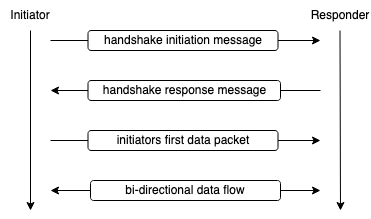
\includegraphics[width=6cm]{paper/images/handshake_process.drawio.png}
\caption{Informal Handshake Narration Process}
\label{fig:handshake_process}
\end{figure}


\label{handshake_message}

\begin{figure}[ht]
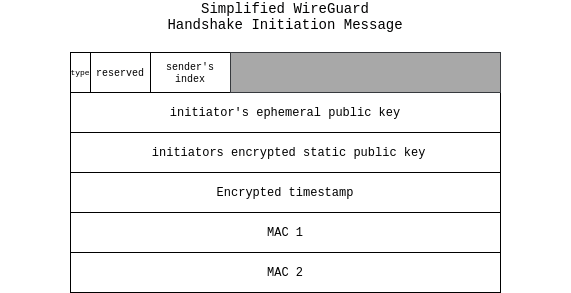
\includegraphics[width=12cm]{paper/images/Wg_hand_init.drawio.png}
\caption{Simplified WireGuard handshake initiation message}
\label{fig:hand_init}
\end{figure}
In the WireGuard protocol, both parties are identified by their static public key's. WireGuard refers to parties as an initiator and a responder, since there is no strict definition of client or server. WireGuard assumes that each party's public key is securely exchanged out-of-band. This exchange must take place before a handshake can be performed. A handshake is performed using an initiation message, sent by the initiator to the responder. The most important fields in the handshake message are shown in Figure \ref{fig:hand_init}.

To create an initiation message, the initiator generates an ephemeral, Curve25519 key-pair. The ephemeral public key is added to the message. The initiator's static public key is encrypted using ChaCha20Poly1350 AEAD. The encryption key for this field is a derived key, which is derived in-part using the responders static public key.
The sender's index is a randomly generated 4-byte value. It is used as a peer's chosen handshake session id.
The responder's public key used as key to MAC 1. This initiation message contains an encrypted form of the initiator's public key.

The contents of the initiation message are authenticated using MAC 1.
A MAC is used to protect the initiation message, with the MAC key being the responders public key.

responder, an initiator is identified by their ability to decrypt messages encrypted with the client's public key, and cannot be revoked, except by manually notifying and removing the client’s public key from all servers. As mentioned previously, in WireGuard, key management is intentionally left up to the users and administrators. There is no certificate revocation mechanism or expiration of client and server keys.

MAC2 is an optional message authentication code and is only used when the anti-DDoS mechanism is enabled for a given responder. While this feature is interesting from the protocol security perspective, further discussion of these features is out of scope for the project.

\section {Identity Portability}
The WireGuard reference implementation doesn't support encrypting a user's private key at rest. The lack of traditional digital certificate support also means a user cannot configure their private key to require a password for use. This forces the user to either generate and share a unique private key for each machine they wish to connect to another WireGuard peer, or manage copying and securely transporting their plain-text private key with them, copying that private key into each machines WireGuard configuration file manually. This process is left up to the user to handle. TODO --move to background

As mentioned previously, WireGuard doesn't support major benefit of WireGuard-HSM's design is that the user's identify becomes physically portable because the private key is securely stored on a USB security key. When using WireGuard-HSM a user is able to securely bring their identify with them and use it on other machines running WireGuard-HSM. 

In contrast, This is a standard feature of most digital certificates.


\section {Contributions}
The Elliptic Curve, Curve25519 is being used in an increasing number of open-source and commercial products\cite{noauthor_things_nodate-1} from SSH to Signal, however hardware support in 
security keys is currently almost non-existent. YubiKey is currently the most popular security key manufacturer however all of their current products 
lack support for X25519. One of the goals of this project, as the first open source project to combine an X25519 supported security key with a popular open source VPN like WireGuard, will encourage more manufactures to add support for X25519 across the security key industry.

\chapter {Related-work}
The WireGuard handshake protocol has gone through extensive formal verification using Tamarin proof system \cite{donenfeld_formal_2018}. Researchers have identified some potential weaknesses in WireGuard around quantum computers but no critical or serious vulnerabilities have been identified since it was introduced five years ago in 2017.

The WireGuard protocol and handshake has been analyzed and dissected without any major flaws discovered. Researchers have demonstrated vulnerabilities might exist for guarantees like perfect-forward-secrecy, if quantum computers can be used to break XXX.  In the area of post-quantum security, a redesign of WireGuard's handshake has been proposed by \cite{hulsing_post-quantum_2021}.
(TODO: ADD IN MORE BG INFORMATION FROM ONE-DRIVE PAPERS AND ADD A BETTER SUMMARY)

\section {Project scope}

My project is focused on improving WireGuard's handling of its private key.
It will be necessary to understand importance of the private key and how it's used during the WireGuard handshake process, when we discuss our threat model in section \ref{wg-ref-analysis}. Next I will discuss some of the features of Curve25519 and its place in WireGuard.


\chapter {Project Background}

12)  2.1 -- Background is more about "what does the reader need to know that I don't expect somebody with a BS or MS in CS to know". Here you should be describing details about curve25519, Nitrokey, pkclient, GnuPG, etc that are relevant to why you did your work the way you did. (Conception)

\section{Configuration}
WireGuard configuration on the command-line is handled via a separate program called wireguard-tools \cite{noauthor_wireguard-tools_2022}. This program handles parsing a plain-text configuration file and turns the configuration directives into API calls to the separately running WireGuard daemon, which configures the virtual-interface. I wanted my program to conform as closely as possible to the WireGuard reference implementation, so I made modifications to the wireguard-tools program. I added support for an 'HSM' line in the plain-text configuration file. 
\begin{figure}[ht]
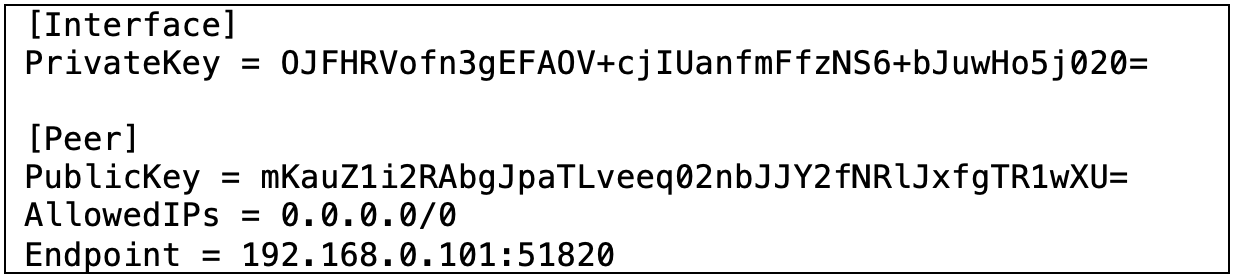
\includegraphics[width=8cm]{paper/images/wg_conf_std.png}
\caption{Example WireGuard Configuration File from the Reference Implementation}
\label{fig:wg_config}
\end{figure}

\begin{figure}[ht]
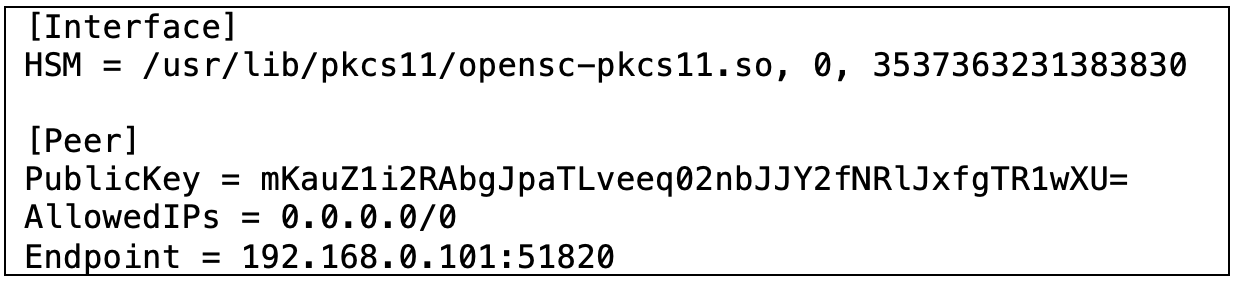
\includegraphics[width=8cm]{paper/images/wg_conf_hsm.png}
\caption{Example WireGuard-HSM Configuration File}
\label{fig:hsm_config}
\end{figure}
This modification removes the requirement for defining and storing the private-key in the plain-text file. The HSM directive tells the program two, and optionally three things. First it lists the PKCS\#11 library path. Second, the slot id  to use on the security key. Thirdly and optionally, the pin required to access the slot.

The detailed workings of the PKCS\#11 interface are out of scope for this paper, however it suffices to say that for interfacing with a security-key, PKCS\#11 requires a slot ID and a secret pin-number for that slot, to enable privileged operations like key-signing or key derivation. The PKCS\#11 interface will inform the caller if they successfully logged into the slot and if the requested operation succeeded or not.

Security is a balancing act between overall system security and user-convenience. Making a system more secure can often come at expense of user-convenience. After writing the initial version of pkclient, I added in the functionality to give the user a choice in saving the pin-number in the configuration or omit it entirely. When the pin is omitted and the configuration file is read to WireGuard-HSM, the program will prompt the user for the pin before the WireGuard interface is configured. If pkclient doesn't have the pin number for the given slot, it cannot be sure the hardware security key is configured properly. Saving the security-key pin-number in the configuration file reduces the security of our system a little and I point this out in the threat model. 

TODO Finish this section?



\chapter {Methodology}

this is where you describe the design of your system and justify your design choices.  Typically this chapter would also include any relevant models that you're using such as the threat model, user model, system model, etc. along with your design goals so that the reader knows exactly what problems you're trying to address and which ones are out of scope.

I will perform a comparative threat model analysis of the reference implementation and WireGuard-HSM. This analysis will show the relative strengths and weaknesses of the designs and what I have improved on.

I will also use some traditional software metrics to evaluate the project.


\section{Compatibility}
Compatibility is an important area of consideration when modifying WireGuard. Since WireGuard has no negotiation of cryptographic primitives, any project that modifies the underlying cryptographic functions or protocol, will introduce client incompatibility, leaving the modified peers only able to communiate with peers of the same type. I designed WireGuard-HSM with this in mind, to allow WireGuard-HSM peers the ability to communicate with unmodified peers.

\section{Security Key}
\begin{figure}[ht]
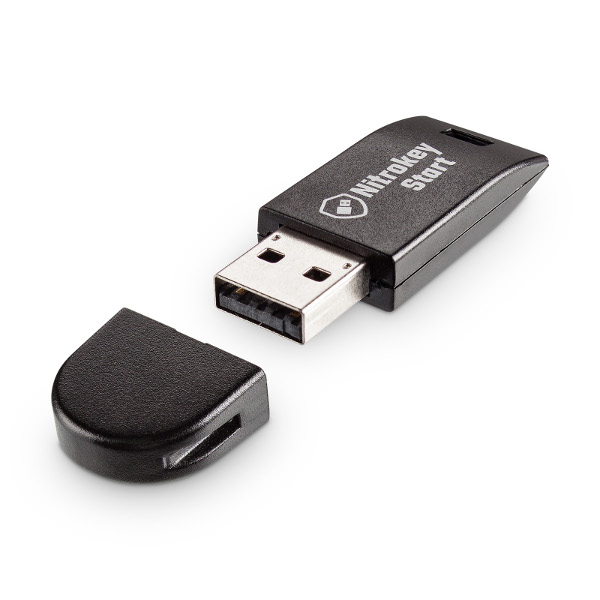
\includegraphics[width=3.5cm]{paper/images/nitrokey.jpg}
\caption{A picture of a NitroKey Start}
\label{nitrokey}
\end{figure}

This distinction is important because WireGuard only uses the X25519 algorithm from Curve25519. Some security keys list support for 'Curve25519' yet most only support Ed25519.

I will give a brief overview of key parts of the NitroKey start. It is hardware security key that connects to a computer via a USB-A interface. It was the only security key at time of writing that supported X25519 operations.
The security key safeguards private keys by allows authenticated users to perform a strict set of key management and cryptographic function on a slot. A slot typically holds private and public keys. The slot is protected by a user PIN. The whole security key itself is protected by a master pin. The master pin is used to unblock a slot, if a user enters a PIN incorrectly three times. After three incorrect guesses the slot is blocked and even the correct PIN will not work on the slot. The slot must be unblocked using the master key, or the device must be erased and reset.

A security key should only be inserted into a computer when its use is required and should be held by the user, on a key chain or other means. Its separation from the computer is important for creating the best security posture. We will discuss the threats that arise when these procedures are not followed by users in section \ref{wg-hsm-analysis}

\chapter {Evaluation}
\section{Threat models analysis}

\subsection {WireGuard - Reference Implementation}
\label{wg-ref-analysis}


Here I present my analysis of the reference implementation of WireGuard. This threat model is focused on WireGuard's asset handling related to the private key, the security controls around it and the threat actors that could be lurking on the system. This computer running WireGuard will be considered Alice's computer and the WireGuard peer Alice connects to is Bob. Alice's computer has been turned on but Alice has not yet established a WireGuard session to Bob's computer. Refer to section \ref{handshake_message} on how WireGuard establishes a peer session. 

\begin{figure}[ht]
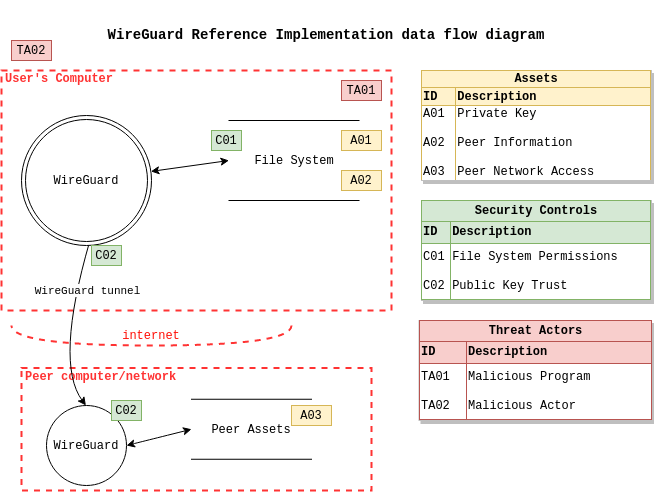
\includegraphics[width=14cm]{paper/images/WG_DFD.drawio.png}
\caption{Threat Model for the WireGuard Reference Implementation - Data Flow Diagram}
\label{fig:wg_ref_dfd}
\end{figure}

\subsection{Assets}
The file system on Alice's computer contains the WireGuard configuration file \ref{fig:wg_config}. 
Asset A01 is Alice's Curve25519 static private key. Asset A02 is Bob's connection information consisting of his Curve25519 static public key and DNS address. It is important to note that in this threat model, both of these assets reside in the same location. Access to the configuration file gives access to both assets.
Asset 03 is the label for any potential assets at the other-side of the WireGuard VPN tunnel. Access to Bob's machine might be a highly valuable asset or Bob's network access might be the highly valuable asset. Our model combines these possibilities into 'Peer Assets' for simplification.

\subsection{Security controls}
Access control in WireGuard's reference implementation for A01 and A02 is C01: proper file system permissions. Most of the documentations (TODO CONFIRM) indicate that the permissions should be set on the WireGuard configuration file to allow only administrator access and restrict access by unprivileged users. For most of the reference implementations that I can find, this is not an enforced measure, meaning WireGuard will still start and not complain if the configuration file permissions are insufficient. 

Access control C02, access to each WireGuard peer, is the public key trust system implemented by WireGuard. See section \ref{handshake_message} for more detail.

\section{Threat Actor 1}
The Primary threat to our system is TA01: a piece of malware that has gained access to Alice's computer by some means. A plausible infection scenario might be that the malware has been delivered to Alice's machine via a compromised website advertisement that is exploiting a new web-browser vulnerability in order to escape the web-browser protections and read files on the local machine.  This malware has been programmed to look for and harvest assets on infected hosts. In our case it will look for common filenames or patterns within files that look like WireGuard configuration files.  
\subsection{Insufficient permissions}
If TA01 gains read-only access a single time to Alice's computer and the file system permissions were not correctly set on the WireGuard configuration file, then the malware gains access to A01 and A02. Access to these assets results in loss of A03 by bypassing C02. See section \ref{impersonation} to see how this works.

\subsection{Sufficient permissions}
If C01 is configured properly, then TA01 will have a more difficult time gaining access to A01 and A02. This offers a single layer of security so TA01 will need to perform a pivot in order to bypass the security control C01. Exploit chains are common-place in today's security field so let's consider an attack that uses more than one vulnerability. Now that TA01 has access to Alice's computer, it will need to pivot in order to bypass C01. I will present three different areas of attack that could be used to pivot. Exploit chaining is a popular technique which could result in one of the following scenarios: gaining administrative privileges, modify file system permissions, trick a privileged process into disclosing the file contents. This is not an exhaustive list of pivots but these three are reasonable scenarios. Once any single one of these pivots is performed, then TA01 has access to A01 and A02 which results in loss of A03 by bypassing C02.

\section{Threat Actor 2}
Our second threat actor is a malicious user who gains direct or indirect access to Alice's computer. 

In a direct method of attack, the second threat actor gains physical access to Alice's laptop and uses some technical or non-technical exploit to read the hard-drive. A technical exploit might be a disk-encryption key recovery vulnerability, allowing TA02 access to the hard drive. TODO expand on this section

The indirect method of attack could be performed by a threat actor using social engineering tactics such as a phone-call masquerading as someone from Alice's IT department, asking her to in some way disclose the contents of the WireGuard configuration file, leading to disclosure of assets A01 and A02.


\subsection{Off-line access}
If Alice's laptop is not protected by hard-drive encryption, then it is trivial for an attacker who has physical access to a laptop to mount and read the contents of the file system on the target device, leading to loss of A01 and A02.

\section{Vulnerabilities}
Once any of the previously weaknesses and have been taken advantage of by a threat, and the threat actor gains access to assets A01 and A02, this creates two different vulnerabilities in our WireGuard system for Alice and Bob. In the CIA model of security, these vulnerabilities threaten confidentially and availability. TODO (define CIA Triad earlier and define impersonation and DOS)
\subsection{Impersonation}
\label{impersonation}
In order to perform a WireGuard handshake as Alice, all a threat actor needs is Alice's private key (A01) and Bob's public key (A02). With these two pieces of information, a threat can now effectively impersonate Alice from any computer in the world, almost undetected. I will discuss how this attack might be detected in the next section \ref{dos}. Loss of A01 and A02 allows for bypassing the public key trust in C02, for any peer found in the configuration file, which is A02. This gives the threat actor access to any assets that are held on Bob's computer or network. VPN's are commonly used as the first layer of defense for network access, so A03 could be access to a network resource that is hidden behind the WireGuard VPN. It is reasonable to assume this attack could also be the first step in an exploit chain to gain access to more assets.
This threatens confidentiality in our system because unauthorized parties can now masquerade as authorized users.

\subsection{Denial-of-Service}
\label{dos}
If asset disclosure is not the goal of an attacker then denial of service is a viable threat to consider. Once a threat can perform impersonation, that can be used to perform a denial of service attack against Alice's WireGuard connection to Bob. When Bob receives and establishes a handshake with Alice's credentials, the initiator established that handshake with a 'sender's index'. This index is a randomly generated 4-byte value which the peer uses to identify the sessions. Once Bob has an established session with Alice's credentials, it will drop any handshake initiations messages that don't contain that index value. In this situation the attacker simply needs to establish a connection before the real Alice does, and Alice will be unable to perform a handshake with Bob until the attacker disconnects.

This denial of service attack would not be noticed by Bob because his WireGuard process thinks he has a legitimate session established with Alice and will silently drop other connection attempts. Alice would only notice that she is unable to establish a session with Bob. Alice would have to communicate with Bob via alternative means, and have him look at his computer's WireGuard session output, then they would need to note that Alice's session is currently established and what remote IP has established the session.

This attack threatens availability in our system because Alice's connection to Bob's resources can be denied by a malicious third-party now.

===================================

\subsection{Threat Modeling System state assumptions}
Assumptions about program and system state. When considering diagramming and system, we need to make several assumptions about the system state. That is, What doe the use case look like? How are the users interacting with the system? What mistakes could the user make when using this system? Does the model we are using capture all of them?
I want to draw attention to key designs about the system and its basic parts related to private key handling.
Alice inserts in the hardware security key when she intends to use WireGuard to connect to Bob. Alice enters her security key pin every time when using it. 

    What would improve this possibility could be using 
XXXY

\section{WireGuard-HSM Threat model}
\label{wg-hsm-analysis}
Threat model analysis of the WireGuard-HSM. This threat model is also focused on WireGuard-HSM's asset handling related to the private key and peer public keys, the security controls around them and possible threat actors to the system. The computer running WireGuard will be considered Alice's computer and the WireGuard peer Alice connects to is referred to as Bob. Alice's computer has been turned on but Alice has not yet established a WireGuard session to Bob's computer. Refer to section \ref{handshake_message} on how WireGuard establishes a peer session. 

\begin{figure}[ht]
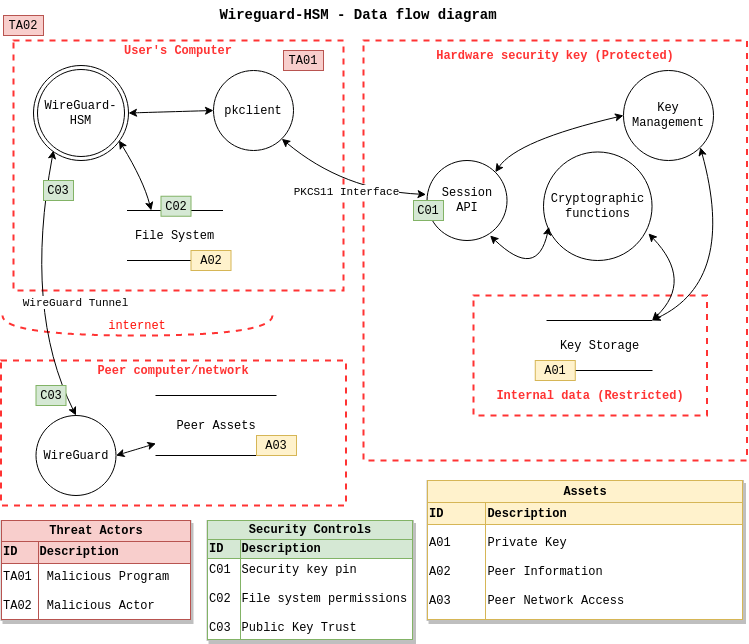
\includegraphics[width=14cm]{paper/images/WGHSM__NoPin_DFD.drawio}
\caption{A Threat Model for WireGuard-HSM - Data Flow Diagram}
\label{fig:wg_hsm_dfd}
\end{figure}

\subsection{Assets}
In this model, the private key asset A01 is completely separated from the peer information asset A02. These assets now resided on physically separate systems. The Peer Assets A03 represent Bob's computer or network access.

\subsection{Security controls}
Access to asset A01 is now behind two layers of defense. Firstly A01 is now on a physically separate system, the hardware security key. Alice must plug in her hardware security key and authenticate with a PIN, Control 01, before cryptographic operations can be performed on A01 via the PKCS\#11 interface with the session API.
File system permissions are used to protect the Peer Information, asset A02.
Security control C03, access to each WireGuard peer, is the public key trust system implemented by WireGuard. See section \ref{handshake_message} for more detail.

\subsection{Use-case Scenario}
To better understand the flow of data and relationships between each part of the diagram, I will describe a use case for WireGuard-HSM.
Alice wants to connect to Bob using WireGuard. Alice logs into her laptop and inserts her security key containing her WireGuard private key. WireGuard reads the configuration file with Bobs public key, sees the HSM directive and loads pkclient. Pkclient prompts Alice to enter her PIN and create an authenticated session with the security key using the PKCS\#11 interface. WireGuard-HSM sends Bob's public key to pkclient as input to the DeriveKey() function on the security key. This function derives a shared key with Alice's private key.

Once WireGuard-HSM receives the derived key from pkclient, it constructs the WireGuard handshake initiation message and sends it to Bob. Bob authenticates the handshake partially on Alice's message

\section{Threat Actor 1}
Let us consider our primary threat, TA01: a piece of malware that has gained access to Alice's computer by some means. A plausible infection scenario might be that the malware has been delivered to Alice's machine via a compromised website advertisement which is exploiting a new web-browser vulnerability in order to escape the web-browser protections and read files on the local machine.  This malware has been programmed to look for and harvest assets on infected hosts. In our case it will look for common filenames or patterns within files, that look like WireGuard configuration files.  

\subsection{Insufficient permissions}
If TA01 gains read-only access a single time to Alice's computer and the file system permissions were not correctly set on the WireGuard configuration file, then the threat gains access to the A02: Peer Information but not A01: Alice's Private key.

\subsection{Sufficient permissions}
If C01: File system permissions, is configured properly, then TA01 will have a difficult time gaining access to A02. This offers a single layer of security, so TA01 will need to perform a pivot in order to bypass the file system permissions. Performing a pivot and gaining access to A02 at this point is less lucrative because A01: Alice's private key is still not accessible to the attacker on this system.

\subsection{Full compromised host}
Let's assume that Alice's computer has been fully compromised by TA01. The malware it has gained persistent, privileged access to Alice's machine. In this scenario, the malware could wait until Alice connects her security key and enters her pin to authenticate WireGuard-HSM to the peer Bob. The malware would have to wait and opportunistically take advantage of Alice's legitimate connection attempts.
WireGuard creates a virtual tunnel that is exposed on the local system as a pseudo-network interface, e.g a TUN interface. Protecting access to the TUN interface is up to the operating system but in this scenario, the fully-compromised host could allow


\section{Threat Actor 2}
Our second threat actor is a malicious user who gains direct or indirect access to Alice's computer. 

In a direct method of attack, the threat actor 02 must gain physical access to Alice's computer and use a technical or non-technical exploit to read the hard-drive. A technical exploit might be a disk-encryption key recovery vulnerability, allowing TA02 access to the hard drive. This will only result in loss A02: Peer Information but A01 is held on Alice's security key which is safely kept on her person.

If Alice left her security key permanently connected to her computer, then there is a risk that the threat actor could gain physical access to both Alice's laptop and her security key. However, the security key is useless, unless the threat actor also learns Alice's PIN. Brute forcing a hardware security key PIN is difficult because a PIN will become blocked after three incorrect guesses.

In the in-direct method of attack, the threat actor must convince Alice through social engineering tactics, to disclose the contents of A02. This information is of limited value because Alice cannot be tricked into disclosing A01. The security key does not allow even authenticated users to export or view a private key.
This attack could still be conceivably possible if Alice was convinced by the threat actor to give away physical possession of her security key. This is a very high bar to reach for a social engineering attack but still possible.


\section{Comparison}
The threats to the WireGuard-HSM system are greatly reduced for Threat Actor 02. Physical access to the machine doesn't yield a successful vulnerability unless Alice leaves her security key with her computer and the attacker has learned her PIN.

Alice's fully compromised system still doesn't pose a threat to A01 because by its design, the Nitrokey Start doesn't allow exporting of private key. A user authenticated or not, cannot read the private key held in the NitroKey's key storage.
WireGuard-HSM decouples two important assets, A01 and A02. A fully compromised host cannot exfiltrate Alice's private key. This system is not vulnerable to a denial of service attack since it requires an external third-party with knowledge of A01 and A02, to impersonate Alice's WireGuard handshake.



== NEEDED? ==
The secrecy of a client's private key is paramount to proper client identification and authorization in WireGuard. WireGuard's design protects many aspects of the key handling that have been error prone in past VPN designs (TODO )
My threat model is based around the secrecy of the private key and reducing the risk found in the reference implementation of WireGuard. Since WireGuard allows clients protected-access to resources across networks, there is value for an attacker to desire access. 
There are two main threats to this privacy.  malware infecting a computer running the reference implementation of WireGuard. The malware could be resident on the computer or it could be a single instance where a browser exploit allows an arbitrary file to be read. Our guards against malware that runs on user's computer and gains access to the plain-text configuration file for WireGuard, leaking the private key which gives the bad-actors the ability to connect to the configured wireguard-peers undetected, as the legitimate user.
== /NEEDED? ==



\section{Performance metrics}

\subsection{Performance}
WireGuard-HSM's use of a USB-connected security key means a small part of its functionality is embedded inside a much less powerful computer than the on running the primary program. I wanted to see what performance impacts this design might introduce to the system. I wanted to also answer the question, would WireGuard-HSM have a user-noticeable impact on performance?

In order to benchmark the performance of the implementations, I added a timing function that saves the current time at the beginning of the sharedSecret() function in WireGuard and DeriveNoise() in pkclient. WireGuard-HSM will still make use of sharedSecret() for ephemeral key operations.
See section \ref{keyflow} for more details on when sharedSecret() is called vs DeriveNoise().

The benchmarks were run on two computers connected via a local Gigabit Ethernet connection. 
WireGuard-HSM ran on a desktop PC running Ubuntu 21.10 configured with an AMD Ryzen 5 2600 CPU @ 3.4GHz nominal speed and 64 GB DDR4 ram. 

The peer computer ran an unmodified WireGuard client included with Ubuntu 21.10 on a machine with an Intel core i5-4590 CPU @ 3.30GHz nominal speed and 16 GB DDR3 ram.  

Each function test was run until 32 function calls had been recorded for the target function, labeled DeriveNoise() for the security key and DeriveSoftware() for the default WireGuard software derive function.
Each test was run 3 times and the results were compiled together for an total of 96 data points for each function. A descriptive statistic analysis performed on the resulting data set.

\begin{figure}
\centering
\begin{minipage}{.5\textwidth}
  \centering
  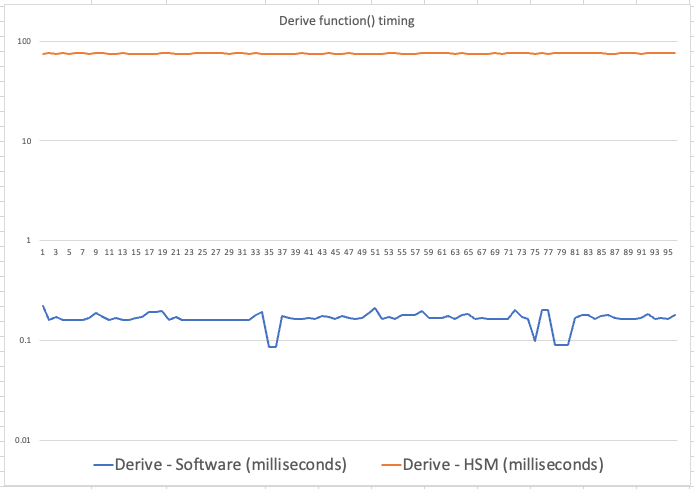
\includegraphics[width=1\linewidth]{paper/images/deriveFunctiongraph.png}
  \caption{Execution Time for DeriveNoise() and softwareDerive()}
  \label{fig:funcTimeGraph}
\end{minipage}%
\begin{minipage}{.5\textwidth}
  \centering
  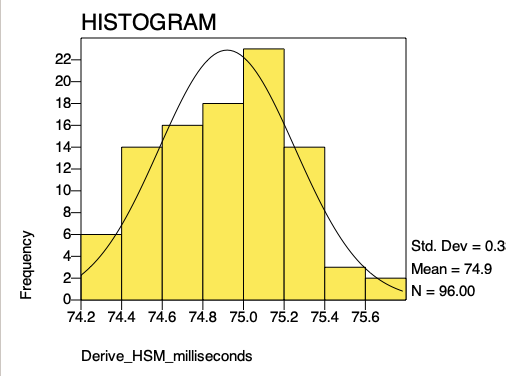
\includegraphics[width=1\linewidth]{paper/images/DeriveNoise freq.png}
  \caption{Histogram of DeriveNoise Execution Time in Milliseconds}
  \label{fig:hsmTimeGraph}
\end{minipage}
\end{figure}

The mean execution time for DeriveHSM() is 74.9 milliseconds and the standard deviation is 0.3 milliseconds. The variance across all data points is .11 milliseconds. 

The mean execution time for softwareDerive() is 0.17 milliseconds and the standard deviation is 0.02 milliseconds. The variance across all data points was too small to be significant.

WireGuard-HSM will use the slower DeriveNoise() when sending a new handshake message or processing a re-key request from a peer. Due to WireGuard's handshake protocol, this will usually happen every 2 minutes. Looking at the performance numbers I can conclude this will add approximately 74 milliseconds of extra processing time each time this function executes. The performance penalty is less than a tenth of a second, so from a human user's perspective, this is almost unnoticeable. 

\chapter {Discussion of Results}
\section {Introduction}
I will discuss the limitations of my project as well as the technical hurdles that I faced while implementing and evaluating my project.

\section{Program Authentication}
One limitation of WireGuard and WireGuard-HSM that can be understood looking at the threat model is that WireGuard operates at the network level, acting as virtual network interface, it makes no guarantees at the operating system level about who or what application is allowed access to the tunnel or not. It is understandable that to maintain platform independence, this is not a goal of the WireGuard project but researchers have proposed a modified WireGuard client that authenticates each application on a smartphone, that is given access to the WireGuard virtual tunnel interface. A major downside of this proposed modification is it requires the user to enter their pin number separately for each application that requires tunnel access, every time WireGuard is started.\cite{wu_sewg_2020}

\section {Limitations}
In this section I will discuss the limitations of my project in regards to the completeness of the evaluation and the limitations of the project implementation itself. Significant time was spent to get the technical implementation of the project working, so I will discuss what improvements I would like to see, if I had more time to complete the evaluation of the entire system.

\subsection{Formal Analysis}
If I had more time, I would include a formal analysis of the security properties of WireGuard-HSM. My goal would be to define WireGuard-HSM in the Tamarin prover to provide a symbolic model of the system. This would show how the security properties of WireGuard-HSM are maintained and provide more proof that the system is secure.

\subsection{Mobile Operating Systems}
I had initially planned to support mobile operating systems such as a smart-phones. Users can easily use security keys
with mobile operating systems but due to technical requirements of the WireGuard protocol, a WireGuard-HSM user would have to leave their security key connected
or after 2\textsuperscript{60} messages are exchanged. This could be avoided by having users modify their WireGuard client and peer defaults to a much longer timeout for re-key, but this seems like a burdensome approach and it may not be possible for the client to request a modification of peer settings.


\section{Compatibility}
WireGuard-HSM is able to perform a successful handshake and pass traffic with an unmodified WireGuard peer.

\chapter {Conclusion}
 
{TODO 15)  In your conclusions section, you mostly focus on future work -- what are the actual conclusions you can draw from the results of your implementation, analysis, and experiments? } 
I have shown that WireGuard-HSM reduces the attack surface for threat actors by moving the long-term static private key into security key. WireGuard-HSM increases the portability of a user's identity while maintaining the security of the private key. This improves the ease-of-use for the user.

\section {Future Work}
There are several areas where I would like to improve WireGuard-HSM that have been identified over the course of implementing and evaluating the system. These areas include pin handling and security key availability and kernel-mode support.

\subsection{Pin handling}
 A user may choose not a save the security-key pin in the WireGuard-HSM configuration file. In this mode, the program must prompt user for the pin. Currently this prompt is very simple and given on the command-line when the user runs WireGuard-HSM. This prompt is easy to miss and wouldn't work very well if WireGuard-HSM was implemented as a kernel module. A better approach would be to have the prompt implemented as a system-dialog window, that appears over any existing windows, making very simple for the user to omit the pin and only enter it when using WireGuard-HSM. Finding a Go-module that opens window dialogues and supports multiple operating system was deemed out of scope for this project but it will be my next addition to the program since it would increase the ease-of-use for the program. 
 
\subsection{Security Key Diversity}
Hardware security-key support for curve25519 and specifically X25519 is, as of writing, very limited. Nitrokey 3 is planned to support X25519 but the hardware is still not in mass production. I would like to see bio-metric hardware-keys with X25519 support, this would add an additional layer of security to our model as it further authenticates the user. As of writing, I could find no planned development for such a key. Many hardware-security keys have introduced support for near-field-communication (NFC) which makes using them with mobile devices almost seamless. Having a security-key with Curve25519 support, would make integrating WireGuard-HSM with mobiles devices easier and put less burden on the user. 

\subsection{Kernel-Mode Support}
WireGuard-HSM is written using the Go language version of WireGuard but a kernel-mode version would be more practical to most users. The Go-version of WireGuard warns users on start-up that if they are on a supported operating system, the kernel version has better support and offers better performance. The main challenge in writing the kernel mode version will be the PKCS\#11 integration and handling user interaction between a kernel module. A small program like pkclient that handled the PKCS\#11 integration and user prompts would be a good first step in expanding the functionality.

\subsection{Bio-metric Authentication}
It would be desirable for this project to use a bio-metric security key for example, a security key that uses a small fingerprint reader to authenticate the user. A bio-metric security key with X25519 support is not yet offered together but they exist in independent implementations, for example Yubico sells a security key that has fingerprint reader needed for user authentication\cite{yubico_yubikey_2022}. 

\chapter{Recycling and Questions}
This will be removed in the final paper, just keeping items here for their reuse

\subsection{questions to answer}
Questions you need to be able to answer by your defense

    What is your contribution? What did you do that is worthy of being an MS Thesis/Capstone?

    What measurements are you taking? Part of your paper will be showing how "good" the system is. What are you using for comparison? How do you know that it is successful?

    What are the limitations? What could be done to improve those if you had more time? 
    What are alternatives decisions you could have made as you developed this and why didn't you choose those options? 
    We want to see that you thought through your work and that you made engineering decisions. 
        This is one of the points of receiving an MS degree is the implication that you have rigorous decision making process within the field of your expertise.
        
\section{Recycling}

\subsection {Conception}
I was interested in WireGuard when it was announced but it wasn't until a group project I started in Winter 2020, where we looked at the security of WireGuard and primarily identified key handling as a potential weak point in the program, that I began to consider different approaches to improving WireGuard,  without introducing a larger attack surface or forking the project. 

In Spring quarter of 2021, I took research methods in software development with Dr Erdly. During this course I continued to explore ideas that I had about WireGuard and its private key handling. I created my final project around WireGuard. In the project, I asked the question, how could WireGuard's private key handling be better? What systems could I create to improve it, and then how could I evaluate those systems?  
In the final part of the project I create a mock survey of software engineers to rate four of the final designs. I used my own metrics to define my terms (TODO finish up this back story, get to point about compatibility)

I came up with three designs that would improve key handling in WireGuard and I rated them on implementation, TODO(dig up project and look at ratings)!! In the end I chose the simplest overall design with the biggest risk being that my design relied on a security key produced by a single manufacture. No other manufacturer at the time sold a security key that supported X25519.

\subsection {Starting out}

I decided to start with interfacing with the NitroKey and getting familiar with the tools and commands to interact with it. I initially chose the Nitrokey start because the product page said it supported X25519\cite{noauthor_nitrokey_nodate} which is the ECDH key derivation process. After a few frustrating days I couldn't figure out how to even generate or put a curve25519 key on the nitrokey start. Searching online, I didn't see any existing software projects that interfaced with a security key for performing X25519 operations. What I did discover after pouring over NitroKey's documentation was that they recommended using a program called OpenSC to work with the Nitrokey but that only a program called GnuPG, when running in an advanced configuration mode, was capable of telling the Nitrokey to generate a set of curve25519 keys. Confusingly, GnuPG can generate the correct keys but it has no ability to perform X25519 with the security key.

\subsection {OpenSC}
Key derivation for ECDH, called X25519 in my specific case when using Curve25519 keys, requires access to Bob's private key and Alice's public key. The cryptographic operation will generate a new 'shared key' that is identical for both parties when the keys are flipped and you use Alice's private key and Bob's public key. 
After researching the OpenSC tool support forums, I was able to find the command string that instructs a  security key to perform the key derivation operation with the correct inputs and outputs. However the tool only produced an error when I tried to use it with the Nitrokey and Alice's public key. I discovered that while NitroKey support documentation says OpenSC is the best tool to use with a Nitrokey Start, OpenSC doesn't support reading curve25519 keys! Why would this key list support for X25519 then? I found out that there was a single test that was written in OpenSC which used the PKCS\#11 interface to generate and verify a shared-secret on the hardware device. This functionality wasn't exposed to users in any way and only ran as part of a test-suite for part of the program. Technically, OpenSC could be used to test that X25519 operations worked on a hardware device but with no user control over the process. This realization set the stage for the rest of the project: technically the functionality is there but no-one has a practical implementation yet. I enjoy a challenge but I was getting worried at this point about the feasibility of completing my project on time.

At this point, I realized that had I created a proof-of-concept program before starting my project, it would have been helpful in gauging how much work this project would entail. It was a frustrating start to my project, I couldn't even start on modifying WireGuard to use the NitroKey if I couldn't find a way to perform X25519.

Analysing the key derivation function in OpenSC and finding the spot where reading my key failed, gave me enough information to start looking into how OpenSC read keys using OpenSSL and then I researched Curve25519 support in OpenSSL. Curve25519 support was a relatively recent addition in version 1.1 of the program\cite{noauthor_support_nodate}.
After digging through the OpenSC tool some more and reading the OpenSSL function documentation, I was able to upgrade how OpenSC read public keys during key derivation and expand its functionality to support X25519 and get the previous command working.
Once I had OpenSC working to perform X25519 on the key, I wrote a test that would perform the operation on the security key and also perform the operation as the other party but in software-only mode, using OpenSSL. The test would verify that the derived key was the same from both steps of the test. This test confirmed that the security key's X25519 function worked correctly and I was finally making progress.

At this point, I realized that all of OpenSC's interaction with the security key is handled via the PKCS\#11 interface and that interface is compiled into a library which connects to the operating system. This library abstracts parts of the lower-level system interactions, so I wouldn't need to worry about, for example, the USB interface. I spent some time looking at how other programs use PKCS\#11 libraries to implement hardware key integration to get more familiar with this area of programming.

\subsection{Interfacing}
At this stage I had X25519 working on the security key and I understood more about PKCS\#11 and how other programs used it. This interfacing part was the area of my proposal that I understood the least. Before I started the project, I wasn't that clear about exactly how I would 'connect' X25519 operations and WireGuard. Using my software development skills that I learned at the UW, I decided it would be best to encapsulate the functionality in a program that would act as the go-between. Handing the various states of the program, user-input and error states. I could create my own limited API for a calling program to request specific actions on the security key. This approach would also reduce the amount of work I would have to do in WireGuard itself.

\subsection{WireGuard Implementation Choice}
I had assumed at the beginning of the project that I should implement my program by modifying the Linux kernel module version of WireGuard. I tried for a few days to learn how to modify and build a kernel module, which has gotten a lot more complicated and time-consuming with things such as module signing and the sheer size of the Linux kernel. I had written and built a kernel module in CSS 537 but that module didn't need to interact with external libraries or handle bi-directional user interactions. After reading the WireGuard kernel module, I decided to try reading through the Go language version of WireGuard. This version is implemented as a standalone program that can run on most operating systems. This version was easier to comprehend and understand the program flow. My project is about implementing new functionality and evaluating the system, so I decided to focus my efforts into modifying the Go version of WireGuard.
The Go programming language has good support for modules which allows programs to easily expand their functionality by importing other code modules. After some more research, I decided to create a Golang module that handled the physical security-key interface and expose a restricted set of functionality to a calling program. 

\subsection{Pkclient}
\label{pk_design}
The most popular and widely-used PKCS\#11 library in Go is called "miekg/pkcs11". From the GitHub repository: "This is a Go implementation of the PKCS\#11 API. It wraps the library closely, but uses Go idiom where it makes sense. It has been tested with SoftHSM."\cite{gieben_pkcs11_2022}. 
I was worried after reading that this program was officially, only tested with SoftHSM, a common software-only version of an HSM. Before I started in earnest, I dug through openly-available public code repositories to try and find an example where someone had used this program to perform key derivation. The only example I could find was another student's class-project where they had evaluated the Go language on aspects related to RSA and ECC key-operations, but had commented out the function on key derivation for unsaid reasons \cite{quapka_go-analysis_2019}. I was worried again starting this phase of the project because it felt very similar to the claims about Nitrokey and X25519: technically this should work but there is no real-world demonstration of the functionality. Would this library actually work with my Nitrokey?

I spent two weeks learning Go language and building and interactively designing a program which I named 'pkclient', to talk to the Nitrokey Start. Pkclient handles logging into the hardware key, prompting the caller for the pin, if the pin is not saved in the configuration file (optional), finding the appropriate X25519-key on the security-key and finally, once properly initialized, pkclient can handle key derivation requests and returning the derived-key back to the caller.


\bibliographystyle{plain}
\bibliography{references}
\end{document}
